\subsection{演化方程}
\label{sec:chap1-evolution-equations}

本节介绍描述流体运动的一组方程. 它们是质量守恒方程, 动量守恒方程以及能量守恒方程. 我们采用运动的 Eulerian 描述, 并限于 Newtonian 流动的情形, 见 Section~\ref{sec:chap1-fundamental-laws}.

本节始终令 $(\Omega_t)_t$ 表示 Definition~\ref{def:chap1-fluid-element} 所定义的任意流体元.

\subsubsection{平衡方程}
\label{subsec:chap1-balance-equations}

\paragraph{质量守恒.}
\label{subsec:chap1-mass-conservation}

回顾我们的假设: 所考察的流动内部既没有物质汇, 也没有物质源. 因此, 质量守恒性质可表述如下: 对任意给定的初始体积 $\Omega_0$, 时刻 $t$ 包含在 $\Omega_t=\varphi_t(\Omega_0)$ 中的物质总质量, 与初始时刻包含在 $\Omega_0$ 中的物质总质量相同.

利用 Definition~\ref{def:chap1-density-field} 中引入的密度概念, 此性质可表示为
\[
  \frac{\mathrm{d}}{\mathrm{d}t}\int_{\Omega_t}\rho\,\mathrm{d}X=0.
\]
为避免方程过于冗长, 除非确有必要, 下文不再写出问题中各未知量对 $(t,X)$ 的依赖关系.

利用输运定理 Theorem~\ref{thm:chap1-transport}, 上式等价于
\[
  \int_{\Omega_t}\left(\frac{\partial\rho}{\partial t}+\operatorname{div}(\rho v)\right)\,\mathrm{d}X=0.
\]
此式必须对任意时刻 $t$ 以及随流动演化的任意流体元 $(\Omega_t)_t$ 成立. 假定 $\rho$ 和 $v$ 是正则函数, 显然得到如下偏微分方程, 它称为质量守恒方程, 连续性方程或质量平衡方程:
\begin{equation}
\label{eq:chap1-mass-balance}
  \frac{\partial\rho}{\partial t}+\operatorname{div}(\rho v)=0.
\end{equation}

\paragraph{线动量方程.}
\label{subsec:chap1-linear-momentum}

本节应用 Newton 第二运动定律来表示流体元 $(\Omega_t)_t$ 的线动量演化. 时刻 $t$ 流体元内包含的总线动量为
\[
  \int_{\Omega_t}\rho v\,\mathrm{d}X.
\]
Newton 第二运动定律指出, 此总动量的变化率等于作用于该流体元的外力之和. 一般而言, 这些力分为两类:
\begin{itemize}
\item 体力
\[
  \int_{\Omega_t}\rho f\,\mathrm{d}X,
\]
其中在许多情形下, 力的质量密度 $f$(表示流体所受的外力)就是重力加速度.
\item 表面力
\[
  \int_{\partial\Omega_t}\tau(\nu)\,\mathrm{d}y,
\]
其中 $\nu$ 是 $\Omega_t$ 的表面 $\partial\Omega_t$ 上指向外部的单位法向量. 这些力由其余流体作用于所考察的流体元 $(\Omega_t)_t$, 称为应力. 向量 $\tau(\nu)$ 当然也依赖于 $(t,y)$, 但方程中未将其明确写出.
\end{itemize}
因此, 一般的线动量方程可利用向量场的输运定理 Remark~\ref{rem:chap1-transport-vector} 写为
\begin{equation}
\label{eq:chap1-linear-momentum-integral}
  \int_{\Omega_t}\left(\frac{\partial(\rho v)}{\partial t}+\operatorname{div}(\rho v\otimes v)\right)\,\mathrm{d}X
  =\int_{\Omega_t}\rho f\,\mathrm{d}X+\int_{\partial\Omega_t}\tau(\nu)\,\mathrm{d}y,
\end{equation}
并且必须对任意流体元 $(\Omega_t)_t$ 成立.

\paragraph{角动量方程.}
\label{subsec:chap1-angular-momentum}

现在把角动量理论应用于流体元 $(\Omega_t)_t$. 该理论指出, 相对于某个给定固定点计算的流体元总角动量的变化率, 等于相对于同一点计算的作用力矩之和.

考虑一个固定点 $O$, 并定义位置向量 $r=\overrightarrow{OX}$, 则可写为
\[
  \frac{\mathrm{d}}{\mathrm{d}t}\int_{\Omega_t}r\wedge(\rho v)\,\mathrm{d}X
  =\int_{\Omega_t}r\wedge(\rho f)\,\mathrm{d}X
  +\int_{\partial\Omega_t}r\wedge\tau(\nu)\,\mathrm{d}y.
\]
由于在 Eulerian 坐标中位置向量 $r$ 不依赖于时间, 输运定理 Theorem~\ref{thm:chap1-transport} 告诉我们, 上式可写成
\[
  \int_{\Omega_t}\left[r\wedge\frac{\partial(\rho v)}{\partial t}
  +\operatorname{div}\bigl((r\wedge\rho v)\otimes v\bigr)\right]\,\mathrm{d}X
  =\int_{\Omega_t}r\wedge(\rho f)\,\mathrm{d}X
  +\int_{\partial\Omega_t}r\wedge\tau(\nu)\,\mathrm{d}y.
\]
此外, 利用\MBUnresolvedReference{eq:app-div-tensor-product}{Appendix~A 中的 Formula~(A.10)}, 有
\begin{align*}
\operatorname{div}\bigl((r\wedge\rho v)\otimes v\bigr)
&=(\operatorname{div}v)(r\wedge\rho v)+(v\cdot\nabla)(r\wedge\rho v)\\
&=r\wedge\bigl((\operatorname{div}v)\rho v\bigr)+\sum_{i=1}^3v_i\partial_{x_i}(r\wedge\rho v)\\
&=r\wedge\bigl((\operatorname{div}v)\rho v\bigr)+\sum_{i=1}^3v_i(r\wedge\partial_{x_i}(\rho v))
 +\sum_{i=1}^3v_i\frac{\partial r}{\partial x_i}\wedge(\rho v)\\
&=r\wedge\bigl((\operatorname{div}v)\rho v\bigr)+r\wedge\bigl(v\cdot\nabla(\rho v)\bigr)
 +\sum_{i=1}^3v_i\frac{\partial r}{\partial x_i}\wedge(\rho v).
\end{align*}
然而, 由于点 $O$ 固定, 有 $\partial r/\partial x_i=e_i$, 其中 $e_i$ 是 $\mathbb{R}^3$ 典范基的第 $i$ 个向量. 因而上式最后一项为
\[
  \sum_{i=1}^3v_i\frac{\partial r}{\partial x_i}\wedge(\rho v)
  =\sum_{i=1}^3v_i e_i\wedge(\rho v)=v\wedge(\rho v)=0.
\]
再次应用该公式, 得
\[
  \operatorname{div}\bigl((r\wedge\rho v)\otimes v\bigr)=r\wedge\operatorname{div}(\rho v\otimes v).
\]
综上, 角动量守恒方程可写成
\begin{equation}
\label{eq:chap1-angular-momentum-integral}
  \int_{\Omega_t}r\wedge\left(\frac{\partial(\rho v)}{\partial t}+\operatorname{div}(\rho v\otimes v)\right)\,\mathrm{d}X
  =\int_{\Omega_t}r\wedge(\rho f)\,\mathrm{d}X
  +\int_{\partial\Omega_t}r\wedge\tau(\nu)\,\mathrm{d}y.
\end{equation}

\paragraph{能量演化.}
\label{subsec:chap1-energy-evolution}

先回顾热力学第一定律: 一个系统总能量的变化率等于机械力的功率与系统同外界热交换率之和.

单位体积的总能量为 $\rho E\equiv\rho(e+\tfrac12|v|^2)$, 其中 $e$ 是与流体热力学状态有关的比内能, 即单位质量的内能, 而 $\tfrac12\rho|v|^2$ 表示单位体积的动能.

外力功率可分解为两项, 一项与体力有关, 另一项与表面上的应力有关:
\[
  \dot W=\int_{\Omega_t}\rho f\cdot v\,\mathrm{d}X
  +\int_{\partial\Omega_t}\tau(\nu)\cdot v\,\mathrm{d}y.
\]
假定体积内部没有热源, 例如辐射热源, 则体积 $\Omega_t$ 中的热输入率具有形式
\[
  \dot Q=-\int_{\partial\Omega_t}\Phi(t,y,\nu)\,\mathrm{d}y,
\]
这里假定跨越 $\Omega_t$ 表面的热传递项 $\Phi$ 仅依赖于位置, 时间以及所考察点处 $\Omega_t$ 的外法向量. 与应力 $\tau$ 一样, 仅在必要时写出其对 $(t,y)$ 的依赖.

能量平衡现在可写为
\[
  \frac{\mathrm{d}}{\mathrm{d}t}\int_{\Omega_t}\rho E\,\mathrm{d}X
  =\int_{\Omega_t}\rho f\cdot v\,\mathrm{d}X
  +\int_{\partial\Omega_t}\tau(\nu)\cdot v\,\mathrm{d}y
  -\int_{\partial\Omega_t}\Phi(\nu)\,\mathrm{d}y.
\]
对时间导数应用输运定理, 得到守恒方程
\begin{equation}
\label{eq:chap1-energy-integral}
  \int_{\Omega_t}\left(\frac{\partial(\rho E)}{\partial t}+\operatorname{div}(\rho E v)\right)\,\mathrm{d}X
  =\int_{\Omega_t}\rho f\cdot v\,\mathrm{d}X
  +\int_{\partial\Omega_t}\tau(\nu)\cdot v\,\mathrm{d}y
  -\int_{\partial\Omega_t}\Phi(\nu)\,\mathrm{d}y.
\end{equation}

\subsubsection{Cauchy 应力定理}
\label{subsec:chap1-cauchy-stress}

本节研究应力 $\tau(\nu)$ 的一般形式, 更确切地说, 证明下面的基本定理. 它指出, 应力关于所考察体积元表面的法向量是线性的. 本节明确写出应力对 $(t,y)$ 的依赖, 因而记作 $\tau(t,y,\nu)$.

\begin{Theorem}[Cauchy's stress]
\label{thm:chap1-cauchy-stress}
假定密度场 $\rho$, 速度场 $v$ 和体力密度 $f$ 是正则的. 另假定当向量 $\nu$ 固定时, 函数 $(t,y)\mapsto\tau(t,y,\nu)$ 连续. 则存在张量值函数 $(t,y)\mapsto\sigma(t,y)$, 使得对所有 $(t,y)$ 和所有单位向量 $\nu$ 都有
\[
  \tau(t,y,\nu)=\sigma(t,y)\cdot\nu.
\]
\end{Theorem}

\begin{Proof}
证明的关键是齐次性论证: 在线动量平衡方程中, 对尺度趋于 $0$ 的基本控制体比较表面积分和体积分的量级. 下面给出计算细节.

首先证明对所有 $(t,y,\nu)$ 都有 $\tau(t,y,\nu)=-\tau(t,y,-\nu)$. 令
\[
  h=\frac{\partial(\rho v)}{\partial t}+\operatorname{div}(\rho v\otimes v)-\rho f,
\]
使得动量守恒方程\eqref{eq:chap1-linear-momentum-integral}对任意区域 $\omega$ 写为
\begin{equation}
\label{eq:chap1-cauchy-control-volume}
  \int_{\omega}h\,\mathrm{d}X=\int_{\partial\omega}\tau(t,y,\nu)\,\mathrm{d}y.
\end{equation}
任取点 $y_0$ 和单位向量 $\nu_0$. 考虑以 $y_0$ 为球心的球 $\omega$, 并以经过 $y_0$ 且垂直于 $\nu_0$ 的平面 $\Sigma$ 将其分成两个半球 $\omega_1$ 和 $\omega_2$, 其中 $\nu_0$ 从 $\omega_1$ 指向 $\omega_2$. 分别对 $\omega$, $\omega_1$ 和 $\omega_2$ 应用上面的守恒方程, 再利用 $\omega=\omega_1\cup\omega_2$ 及其边界的相应分解, 得
\[
  \int_{\partial\omega_1\cap\Sigma}\bigl(\tau(t,y,\nu_0)+\tau(t,y,-\nu_0)\bigr)\,\mathrm{d}y=0.
\]
此式对以 $y_0$ 为球心且任意小的球均成立. 由 $y\mapsto\tau(t,y,\nu_0)+\tau(t,y,-\nu_0)$ 的连续性, 得
\[
  \tau(t,y_0,-\nu_0)=-\tau(t,y_0,\nu_0).
\]

函数 $\tau(t,y,\nu)$ 先验地仅对单位向量 $\nu$ 定义. 利用上述性质, 可将其延拓到 $\mathbb{R}^3$ 的所有向量 $\xi$:
\[
  \tau(t,y,\xi)=|\xi|\tau\left(t,y,\frac{\xi}{|\xi|}\right),\qquad
  \tau(t,y,0)=0.
\]
由此可见该函数关于 $\xi$ 是一阶齐次的. 对任意 $\lambda$, 有
\[
\tau(t,y,\lambda\xi)=|\lambda||\xi|\tau\left(t,y,\frac{\lambda\xi}{|\lambda\xi|}\right)
=|\lambda||\xi|\tau\left(t,y,\operatorname{sgn}(\lambda)\frac{\xi}{|\xi|}\right)
=\lambda\tau(t,y,\xi).
\]

下面证明函数 $\xi\mapsto\tau(t,y,\xi)$ 的可加性. 取 $\xi_1,\xi_2\in\mathbb{R}^3$. 若它们共线, 上述齐次性足以得到结论. 现设 $\xi_1$ 与 $\xi_2$ 不共线, 并固定点 $y_0$. 由点 $y_0$ 和向量 $\xi_1,\xi_2$ 生成一个定向平面 $\mathcal P$, 这等价于选择该平面的单位法向量 $\nu_0$. 记 $\xi_i^\perp$ 为将 $\xi_i$ 沿正向旋转 $\pi/2$ 所得到的向量.

\begin{figure}[htbp]
  \centering
  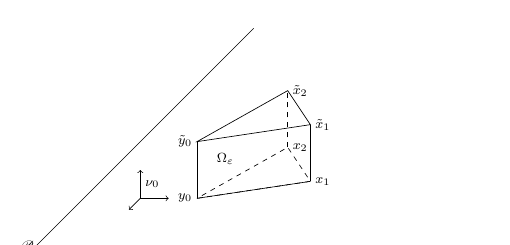
\includegraphics[width=.58\linewidth]{figures/ch01-prism.png}
  \caption{棱柱 $\Omega_\varepsilon$}
  \label{fig:chap1-cauchy-prism}
\end{figure}

引入点
\[
  x_1=y_0+\varepsilon\xi_1^\perp,\qquad x_2=y_0-\varepsilon\xi_2^\perp,
\]
以及
\[
  \widetilde y_0=y_0+\varepsilon\nu_0,\qquad
  \widetilde x_1=x_1+\varepsilon\nu_0,\qquad
  \widetilde x_2=x_2+\varepsilon\nu_0.
\]
于是 $y_0x_1x_2\widetilde y_0\widetilde x_1\widetilde x_2$ 构成高度为 $\varepsilon$ 且以三角形 $y_0x_1x_2$ 为底面的直棱柱 $\Omega_\varepsilon$, 见 Figure~\ref{fig:chap1-cauchy-prism} 和 Figure~\ref{fig:chap1-cauchy-triangle}. 将式\eqref{eq:chap1-cauchy-control-volume}应用于 $\Omega_\varepsilon$ 并除以 $\varepsilon^2$, 得
\begin{equation}
\label{eq:chap1-cauchy-scaled-balance}
  \frac1{\varepsilon^2}\int_{\Omega_\varepsilon}h\,\mathrm{d}X
  =\frac1{\varepsilon^2}\int_{\partial\Omega_\varepsilon}\tau(t,y,\nu)\,\mathrm{d}y.
\end{equation}

\begin{figure}[htbp]
  \centering
  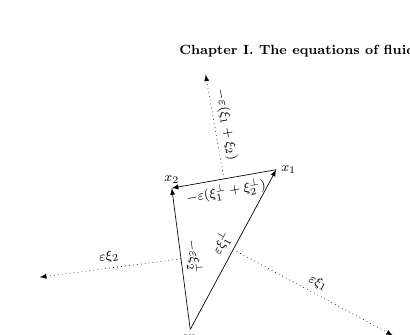
\includegraphics[width=.50\linewidth]{figures/ch01-triangle.png}
  \caption{平面 $\mathcal P$ 中的三角形 $y_0x_1x_2$}
  \label{fig:chap1-cauchy-triangle}
\end{figure}

表面项分成五部分: 三个棱柱侧面和两个底面. 两个底面的外单位法向量为 $\pm\nu_0$, 侧面的外单位法向量与平面 $\mathcal P$ 中三角形 $y_0x_1x_2$ 的外单位法向量相同. 因为
\[
  x_1-y_0=\varepsilon\xi_1^\perp,\qquad
  x_2-y_0=-\varepsilon\xi_2^\perp,\qquad
  x_2-x_1=-\varepsilon(\xi_1^\perp+\xi_2^\perp),
\]
所以存在与 $\varepsilon$ 无关的 $\eta\in\{-1,1\}$, 使三个侧面的外单位法向量依次为
\[
  \eta\frac{\xi_1}{|\xi_1|},\qquad
  \eta\frac{\xi_2}{|\xi_2|},\qquad
  -\eta\frac{\xi_1+\xi_2}{|\xi_1+\xi_2|}.
\]
利用 $\tau$ 关于 $\xi$ 的齐次性, 式\eqref{eq:chap1-cauchy-scaled-balance}右端可写为
\begin{align*}
&-\frac{\eta}{\varepsilon^2|\xi_1+\xi_2|}
\int_{x_1x_2\widetilde x_2\widetilde x_1}\tau(t,y,\xi_1+\xi_2)\,\mathrm{d}y\\
&+\frac{\eta}{\varepsilon^2|\xi_1|}
\int_{y_0x_1\widetilde x_1\widetilde y_0}\tau(t,y,\xi_1)\,\mathrm{d}y
+\frac{\eta}{\varepsilon^2|\xi_2|}
\int_{y_0x_2\widetilde x_2\widetilde y_0}\tau(t,y,\xi_2)\,\mathrm{d}y\\
&+\frac1{\varepsilon^2}\int_{y_0x_1x_2}\tau(t,y,-\nu_0)\,\mathrm{d}y
+\frac1{\varepsilon^2}\int_{\widetilde y_0\widetilde x_1\widetilde x_2}\tau(t,y,\nu_0)\,\mathrm{d}y.
\end{align*}
两个底面的面积相等, 均为 $\varepsilon^2|\xi_1\wedge\xi_2|/2$. 由 $\tau(t,y,-\nu_0)=-\tau(t,y,\nu_0)$, 连续性和积分中值定理, 两个底面项之和在 $\varepsilon\to0$ 时趋于 $0$. 每个矩形侧面的面积为相应的 $\varepsilon^2|\xi_i|$, 连续性保证三个侧面项分别趋于 $\eta\tau(t,y_0,\xi_1)$, $\eta\tau(t,y_0,\xi_2)$ 和 $-\eta\tau(t,y_0,\xi_1+\xi_2)$.

最后考察式\eqref{eq:chap1-cauchy-scaled-balance}中的体积项. 根据假设, $\rho$ 和 $v$ 是正则场, 因而 $h$ 局部有界. 棱柱 $\Omega_\varepsilon$ 的体积与 $\varepsilon^3$ 成正比, 所以
\[
  \frac1{\varepsilon^2}\left|\int_{\Omega_\varepsilon}h\,\mathrm{d}X\right|
  \leq C\varepsilon\longrightarrow0.
\]
令 $\varepsilon\to0$, 得
\[
  0=\eta\tau(t,y_0,\xi_1)+\eta\tau(t,y_0,\xi_2)-\eta\tau(t,y_0,\xi_1+\xi_2),
\]
即
\[
  \tau(t,y_0,\xi_1+\xi_2)=\tau(t,y_0,\xi_1)+\tau(t,y_0,\xi_2).
\]
以上论证证明了应力 $\tau(t,y,\xi)$ 关于 $\xi$ 的线性, 因而证明存在张量 $\sigma(t,y)$, 使每个单位向量 $\nu$ 都满足 $\tau(t,y,\nu)=\sigma(t,y)\cdot\nu$.
\end{Proof}

\begin{Definition}
\label{def:chap1-stress-tensor}
对每个点 $(t,y)$, 由关系
\[
  \tau(t,y,\nu)=\sigma(t,y)\cdot\nu,\qquad\text{对所有单位向量 $\nu$},
\]
定义的张量 $\sigma(t,y)$ 称为流动的应力张量.
\end{Definition}

为避免方程冗长, 下文不再标明应力张量对 $(t,y)$ 的依赖, 并把应力写为 $\tau(\nu)=\sigma\cdot\nu$. 利用散度定理, 即 Stokes 公式\MBUnresolvedReference{thm:stokes-formula}{Theorem~III.1.8}, 能量守恒方程\eqref{eq:chap1-energy-integral}中的表面项可写为
\[
  \int_{\partial\Omega_t}(\sigma\cdot\nu)\cdot v\,\mathrm{d}y
  =\int_{\partial\Omega_t}\nu\cdot({}^{t}\!\sigma\cdot v)\,\mathrm{d}y
  =\int_{\Omega_t}\operatorname{div}({}^{t}\!\sigma\cdot v)\,\mathrm{d}X.
\]
因此, 能量演化方程变为
\begin{equation}
\label{eq:chap1-energy-stress-integral}
\int_{\Omega_t}\left(\frac{\partial(\rho E)}{\partial t}+\operatorname{div}(\rho E v)\right)\,\mathrm{d}X
=\int_{\Omega_t}\rho f\cdot v\,\mathrm{d}X
+\int_{\Omega_t}\operatorname{div}({}^{t}\!\sigma\cdot v)\,\mathrm{d}X
-\int_{\partial\Omega_t}\Phi(\nu)\,\mathrm{d}y.
\end{equation}

现在可以对热传递项 $\Phi$ 建立一个与 Cauchy 定理类似的结果.

\begin{Theorem}
\label{thm:chap1-heat-flux}
假定 $\rho$, $E$, $v$ 和 $f$ 是正则函数. 进一步假定对每个 $\nu$, 函数 $(t,y)\mapsto\Phi(t,y,\nu)$ 连续. 则存在连续向量场 $\phi$, 使得
\[
  \Phi(t,y,\nu)=\phi(t,y)\cdot\nu.
\]
\end{Theorem}

此向量场称为流动中的热通量. 该结果的证明与 Cauchy 定理的证明在形式上完全相同, 只需使用形式为\eqref{eq:chap1-energy-stress-integral}的能量守恒方程. 再次应用散度定理, 得
\[
\int_{\Omega_t}\left(\frac{\partial(\rho E)}{\partial t}+\operatorname{div}(\rho E v)\right)\,\mathrm{d}X
=\int_{\Omega_t}\rho f\cdot v\,\mathrm{d}X
+\int_{\Omega_t}\operatorname{div}({}^{t}\!\sigma\cdot v)\,\mathrm{d}X
-\int_{\Omega_t}\operatorname{div}\phi\,\mathrm{d}X.
\]
由于此式对随流动演化的任意流体元 $(\Omega_t)_t$ 成立, 得到局部形式
\begin{equation}
\label{eq:chap1-energy-local}
  \frac{\partial(\rho E)}{\partial t}+\operatorname{div}(\rho E v)
  -\operatorname{div}({}^{t}\!\sigma\cdot v)+\operatorname{div}\phi=\rho f\cdot v.
\end{equation}

\subsubsection{重新考察演化方程}
\label{subsec:chap1-evolution-revisited}

由 Cauchy 定理可知应力具有张量形式 $\tau(\nu)=\sigma\cdot\nu$, 因而可推导出动量守恒方程的较简单形式. 散度定理\MBUnresolvedReference{thm:stokes-formula}{Theorem~III.1.8} 告诉我们, 对任意区域 $\Omega$,
\[
  \int_{\partial\Omega}\sigma\cdot\nu\,\mathrm{d}y=\int_\Omega\operatorname{div}\sigma\,\mathrm{d}X.
\]
因此式\eqref{eq:chap1-linear-momentum-integral}可写为
\[
\int_{\Omega_t}\left(\frac{\partial(\rho v)}{\partial t}+\operatorname{div}(\rho v\otimes v)\right)\,\mathrm{d}X
=\int_{\Omega_t}\rho f\,\mathrm{d}X+\int_{\Omega_t}\operatorname{div}\sigma\,\mathrm{d}X.
\]
此关系必须对任意流体元成立, 因而得到线动量方程的局部形式
\begin{equation}
\label{eq:chap1-linear-momentum-local}
  \frac{\partial(\rho v)}{\partial t}+\operatorname{div}(\rho v\otimes v)-\operatorname{div}\sigma=\rho f.
\end{equation}

下面考察角动量守恒关系. 先计算表面项, 并尝试将 $r\wedge(\sigma\cdot\nu)$ 写成 $T\cdot\nu$ 的形式, 其中 $T$ 是待定张量. 对典范基的第 $i$ 个向量, 有
\begin{align*}
r\wedge(\sigma\cdot e_i)
&=(r_2\sigma_{3i}-r_3\sigma_{2i})e_1
 +(r_3\sigma_{1i}-r_1\sigma_{3i})e_2
 +(r_1\sigma_{2i}-r_2\sigma_{1i})e_3.
\end{align*}
这表明张量矩阵 $T$ 的第 $i$ 列为
\[
  \begin{pmatrix}r_2\sigma_{3i}-r_3\sigma_{2i}\\r_3\sigma_{1i}-r_1\sigma_{3i}\\r_1\sigma_{2i}-r_2\sigma_{1i}\end{pmatrix}.
\]
对 $T$ 应用散度定理, 式\eqref{eq:chap1-angular-momentum-integral}中的表面项成为体积分, 从而得到角动量方程的局部形式
\begin{equation}
\label{eq:chap1-angular-momentum-local}
  r\wedge\left(\frac{\partial(\rho v)}{\partial t}+\operatorname{div}(\rho v\otimes v)-\rho f\right)-\operatorname{div}T=0.
\end{equation}

利用 $\partial r_i/\partial x_j=\delta_{ij}$, 计算 $T$ 的散度. 例如第一分量为
\begin{align*}
(\operatorname{div}T)_1
&=\sum_{i=1}^3\frac{\partial}{\partial x_i}(r_2\sigma_{3i}-r_3\sigma_{2i})\\
&=\sum_{i=1}^3\left(r_2\frac{\partial\sigma_{3i}}{\partial x_i}-r_3\frac{\partial\sigma_{2i}}{\partial x_i}\right)
+\sum_{i=1}^3\left(\frac{\partial r_2}{\partial x_i}\sigma_{3i}-\frac{\partial r_3}{\partial x_i}\sigma_{2i}\right)\\
&=(r\wedge\operatorname{div}\sigma)_1+(\sigma_{32}-\sigma_{23}).
\end{align*}
另外两个分量的类似计算给出
\[
  \operatorname{div}T=r\wedge\operatorname{div}\sigma
  +\begin{pmatrix}\sigma_{32}-\sigma_{23}\\\sigma_{13}-\sigma_{31}\\\sigma_{21}-\sigma_{12}\end{pmatrix}.
\]
因此式\eqref{eq:chap1-angular-momentum-local}可写成
\[
r\wedge\left(\frac{\partial(\rho v)}{\partial t}+\operatorname{div}(\rho v\otimes v)-\rho f-\operatorname{div}\sigma\right)
-\begin{pmatrix}\sigma_{32}-\sigma_{23}\\\sigma_{13}-\sigma_{31}\\\sigma_{21}-\sigma_{12}\end{pmatrix}=0.
\]
由式\eqref{eq:chap1-linear-momentum-local}, 上式中的向量积恒为零. 因而
\[
  \begin{pmatrix}\sigma_{32}-\sigma_{23}\\\sigma_{13}-\sigma_{31}\\\sigma_{21}-\sigma_{12}\end{pmatrix}=0.
\]
这一基本性质可表述如下.

\begin{Theorem}
\label{thm:chap1-symmetric-stress}
假定密度场 $\rho$, 速度场 $v$ 和体力场 $f$ 光滑. 则作用于流动中流体的应力张量是对称的.
\end{Theorem}

此结果有若干基本推论. 其中之一是: 对每个点 $(t,y)$, 存在 $\mathbb{R}^3$ 的一个标准正交基, 使张量 $\sigma$ 对角化. 这些基向量称为张量的主轴, 相应的特征值称为与张量 $\sigma$ 相关的主应力.
